\documentclass[border=3pt]{standalone}
\usepackage{tikz}
\usetikzlibrary{arrows.meta,calc,positioning}
\tikzset{pin/.style={-{Stealth[length=5pt]}},
  pg/.style={draw, thick, minimum width=16mm, minimum height=10mm, font=\sffamily\small},
  cl/.style={draw, thick, minimum width=76mm, minimum height=12mm, font=\sffamily\small}}
\begin{document}
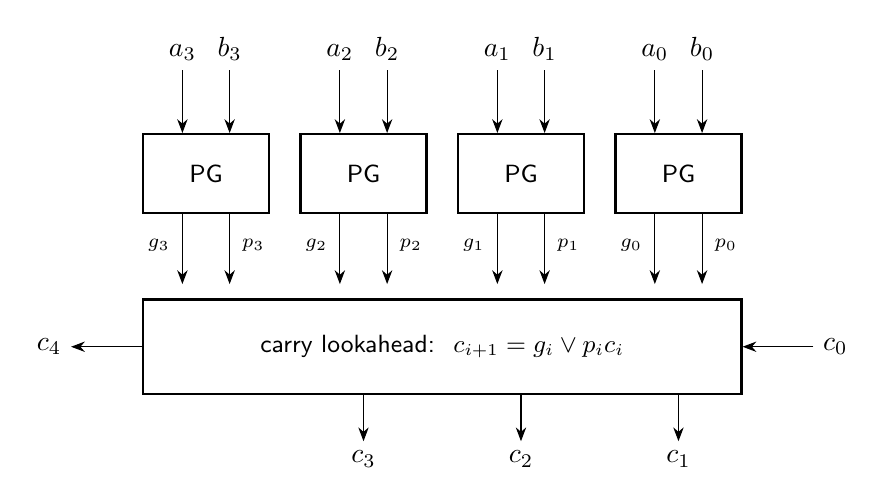
\begin{tikzpicture}[font=\sffamily]
  % PG blocks, bit 0 rightmost
  \foreach \x/\i in {0/0,-2/1,-4/2,-6/3}{
    \node[pg] (p\i) at (\x,0) {PG};
    \draw[pin] ($(p\i.north)+(-3mm,8mm)$) node[above]{$a_\i$} -- ($(p\i.north)+(-3mm,0)$);
    \draw[pin] ($(p\i.north)+(3mm,8mm)$) node[above]{$b_\i$} -- ($(p\i.north)+(3mm,0)$);}
  % lookahead unit
  \node[cl] (cl) at (-3,-2.2) {carry lookahead:\; $c_{i+1} = g_i \lor p_i c_i$};
  % g,p arrows down
  \foreach \i in {0,1,2,3}{
    \draw[pin] ($(p\i.south)+(-3mm,0)$) -- ($(p\i.south)+(-3mm,-8.9mm)$);
    \draw[pin] ($(p\i.south)+(3mm,0)$) -- ($(p\i.south)+(3mm,-8.9mm)$);
    \node[font=\sffamily\scriptsize] at ($(p\i.south)+(-6mm,-4mm)$) {$g_\i$};
    \node[font=\sffamily\scriptsize] at ($(p\i.south)+(6mm,-4mm)$) {$p_\i$};}
  % carry in / out
  \draw[pin] ($(cl.east)+(9mm,0)$) node[right]{$c_0$} -- (cl.east);
  \draw[pin] (cl.west) -- ++(-9mm,0) node[left]{$c_4$};
  % carries out the bottom
  \foreach \x/\i in {0/1,-2/2,-4/3}{
    \draw[pin] (\x,-2.8) -- ++(0,-6mm) node[below]{$c_\i$};}
\end{tikzpicture}
\end{document}
